\section{Data structure}
ALG-3D is a graph-based data structure used to represent a
three-dimensional domain which supports adaptive refinement. For
ease of presentation, the implementation in this paper is based on a
unit cube, although any arbitrary solid region could be used.

\subsection{Concepts}
Start with a unit cube centered at the point $(1/2,1/2,1/2)$, so
that it is entirely contained in the first octant of the standard
$xyz$ coordinate system. Create an initial mesh by uniformly
dividing this cube into eight smaller cubic cells of length $1/2$.
These eight cells are centered at the points $(1/4,1/4,1/4)$,
$(1/4,1/4,3/4)$, $(1/4,3/4,1/4)$, $(1/4,3/4,3/4)$, $(3/4,3/4,1/4)$,
$(3/4,3/4,3/4)$, $(3/4,1/4,1/4)$ and $(3/4,1/4,3/4)$, as shown in
Figure \ref{FIG_INITIAL_GRAPH_MESH}(b). Each of these initial eight
cells is identified according to the position it occupies in the
mesh. The cell in the upper right corner of the frontal face of the
mesh (meaning the face of the cube pointing in the positive
$x$-direction), whose center is $(3/4,3/4,3/4)$, is called the front
northeast cell. The remaining cells in the frontal face are,
counterclockwise: front northwest, front southwest and front
southeast. The cells of the back face of the mesh (closer to the
$yz$ plane) are, counterclockwise: back northeast, back northwest,
back southwest and back southeast.

%Graph and initial mesh
\begin{figure}[!ht]
    \centering
    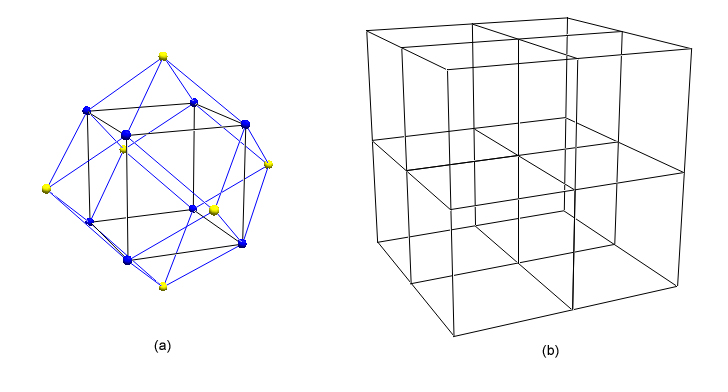
\includegraphics[scale=0.37,angle=0]{../img/initialGraphAndGrid.jpg}
    \caption{Initial mesh and its associated graph.}
    \label{FIG_INITIAL_GRAPH_MESH}
\end{figure}


Associated to this initial division of the unit cube into eight
equal cubic cells is an initial graph (Figure
\ref{FIG_INITIAL_GRAPH_MESH}(a)). To each cell corresponds a
\textit{cell node} in the graph (dark colored in Figure
\ref{FIG_INITIAL_GRAPH_MESH}(a)). Each cell node stores any
information associated to the cell it represents in variables, such
as the spatial coordinates of its centers and physical states (if
the numerical simulation of a physical phenomenon is intended; their
number varies according to the problem being considered). Each of
the eight cell nodes in Figure \ref{FIG_INITIAL_GRAPH_MESH}(a) has
six links oriented along the six directions: \textit{east}, along
positive $y$ direction; \textit{west}, along negative $y$ direction;
\textit{north}, along positive $z$ direction; \textit{south}, along
negative $z$ direction; \textit{front}, along positive $x$
direction, and \textit{back}, along negative $x$ direction. In the
computer code, these six links are six pointers.

Each cell node has also two special pointers called \textit{next}
and \textit{previous}. These pointers are used for ordering the cell
nodes in the graph. Since the graph can become very irregular after
successive refinements of different depths in different regions of
the domain, it can become very difficult to visit the cells in a
systematic way. This auxiliary chain list facilitates the access to
the graph cell nodes, independently of any topological configuration
the graph may assume. The maintenance of this list and the
definition of the order of each cell node in it is done by the
Hilbert curve, as will be explained in detail in Section
\ref{SEC_HILBERT_CURVE}.

The cell nodes also possess a variable that stores its current
refinement level. When a cell node of level $n$ is refined, its
eight daughter cells will each have level $n+1$. After a
derefinement, the opposite happens: eight cells of level $n$ fuse in
order to constitute a cell of level $n-1$.

In the graph structure underlying ALG there is another type of node
called a \textit{transition node}, which is used to connect cell
nodes of different refinement levels. Each transition node has five
links: one single connector and four quadruple connectors. These
five links are implemented as five pointers in the computer code.
They too are assigned variables corresponding to their refinement
levels. In order to better understand the purpose of these
transition nodes, consider the graph in Figure
\ref{FIG_REFINED_GRAPH}, which has a bunch of eight cells with one
level of refinement higher than the refinement level of the initial
cells.

%INITIAL GRAPH
\begin{figure}[H]
    \centering
    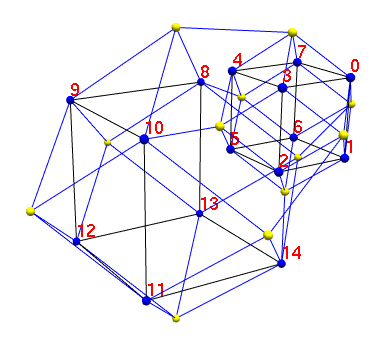
\includegraphics[scale=0.6,angle=0]{../img/refinedGraph.jpg}
    \caption{Communication between cell nodes and transition nodes.}
    \label{FIG_REFINED_GRAPH}
\end{figure}

Cell nodes $2$, $3$, $4$ and $5$ have cell node $10$ as the neighbor
in the west direction. Reciprocally, cell node $10$ has cell nodes
$2$, $3$, $4$ and $5$ as its neighbors in the east direction. Cell
nodes $2$, $3$, $4$ and $5$ could point their respective west
pointers to cell node $10$, but there is no way cell node $10$ can
point its only east pointer to the four neighbor cells
simultaneously. For this reason, a transition node has been created
in order to handle the communication between these nodes. Thus, the
east pointer of cell node $10$ is pointed to the transition node,
whose four quadruple connectors points each to each of the four cell
nodes $2$, $3$, $4$ and $5$. The single connector of the transition
node is pointed to cell node $10$ and the west pointer of each of
the nodes $2$, $3$, $4$ and $5$ is pointed to the transition node.

\subsection{Implementation}
The implementation chosen in this paper is based on the
object-oriented programming paradigm. The class \textit{Cell}
represents the nodes of the graph, irrespective of their types.
Since there are two different types of nodes, two inherited classes
were created: class \textit{CellNode} represents the cell nodes and
class \textit{TransitionNode} represents the transition nodes. See
Figure \ref{FIG_CELL_DIAGRAM}.

%CLASSES Cell, CellNode e TransitionNode
\begin{figure}[H]
    \centering
    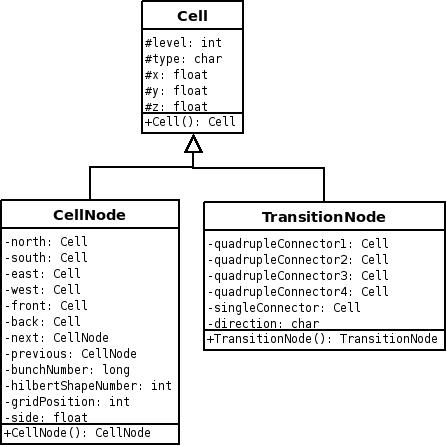
\includegraphics[scale=0.48,angle=0]{../img/cellDiagram.jpg}
    \caption{Hierarchy of classes Cell, CellNode and TransitionNode.}
    \label{FIG_CELL_DIAGRAM}
\end{figure}

The ALG graph itself is encapsulated by the class \textit{Grid}. The
refinement and derefinement methods, as well as other methods of
internal use for the maintenance of the data structure, are
implemented as members of this class (see Figure
\ref{FIG_GRID_DIAGRAM}).

%CLASS Grid
\begin{figure}[!ht]
    \centering
    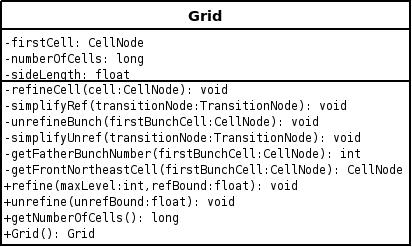
\includegraphics[scale=0.48,angle=0]{../img/gridDiagram.jpg}
    \caption{Class Grid.}
    \label{FIG_GRID_DIAGRAM}
\end{figure}

When an object of type \textit{Grid} is instantiated, the
constructor generates an initial graph as the one of Figure
\ref{FIG_INITIAL_GRAPH_MESH}. The steps necessary for the creation
of this initial graph are described by the algorithm
\ref{CONSTRUCTOR}.

\alglanguage{pseudocode}
\begin{algorithm}[!ht]
    \caption{Steps followed by the constructor of class Grid in order to create the initial graph.}
    \small{
    \begin{algorithmic}[1]
            \State Create eight cell nodes.
            \State Create six transition nodes.
            \State $sideLength \gets 1$

            \State
            \For{\textbf{each} cell node}
                \State Compute and set current node's coordinates.
                \State Points each current node's directional pointers to appropriate cell.
                \State Set current node's previous and next pointers according to Hilbert curve's ordering.
                \State Set current node's level to one.
                \State Set current node's side to $sideLength / 2$.
                \State Initialize other attributes pertinent to the current application.
            \EndFor

            \State
            \For{\textbf{each} transition node}
                \State Compute and set current node's coordinates.
                \State Point each current node's quadruple connector to appropriate cell node.
                \State Set current node's single connector to null.
                \State Set current node's level to one.
            \EndFor

            \State
            \State $numberOfCells \gets 8$.
            \State Set pointer $firstCell$ to the first cell of the Hilbert Curve list.
    \end{algorithmic} \label{CONSTRUCTOR}
    }
\end{algorithm}

The remaining members of class \textit{Grid}, which perform the
functions of refinement, derefinement and ordering of the cell nodes
via the Hilbert curve, will be discussed in the next sections.
